% 图 6.7 一维伊辛模型（按原书 116 页样式：纯箭头字符，无格点圆圈、无畴壁线）
% (a) 基态 N+1 个自旋全部向上 (b) 单个缺陷：前两格向上其余向下
\documentclass[tikz,border=5pt]{standalone}
\usetikzlibrary{arrows.meta}
\usepackage{amsmath}
\usepackage{bm}
\usepackage{fontspec}
\setmainfont{Times New Roman}
\begin{document}
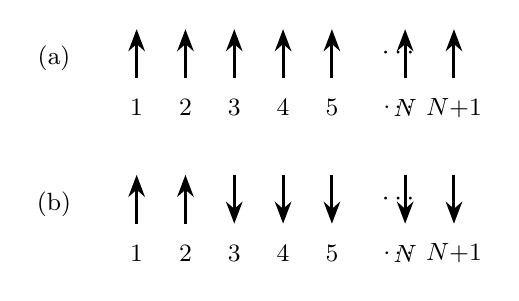
\begin{tikzpicture}[>=Stealth,line width=1.1pt]
\def\dx{0.62}
% ---- (a) ----
\node[font=\small] at (-1.05,0.35) {(a)};
\foreach \i in {0,...,4}{
  \draw[->] ({\i*\dx},0.10) -- ({\i*\dx},0.72);}
\node at (3.35,0.41) {$\cdots$};
\draw[->] ({5.5*\dx},0.10) -- ({5.5*\dx},0.72);
\draw[->] ({6.5*\dx},0.10) -- ({6.5*\dx},0.72);
\foreach \i/\t in {0/1,1/2,2/3,3/4,4/5}{
  \node[font=\small] at ({\i*\dx},-0.28) {$\t$};}
\node[font=\small] at (3.35,-0.28) {$\cdots$};
\node[font=\small] at ({5.5*\dx},-0.28) {$N$};
\node[font=\small] at ({6.5*\dx},-0.28) {$N{+}1$};
% ---- (b) ----
\begin{scope}[shift={(0,-1.85)}]
\node[font=\small] at (-1.05,0.35) {(b)};
\draw[->] (0,0.10) -- (0,0.72);
\draw[->] (\dx,0.10) -- (\dx,0.72);
\foreach \i in {2,3,4}{
  \draw[->] ({\i*\dx},0.72) -- ({\i*\dx},0.10);}
\node at (3.35,0.41) {$\cdots$};
\draw[->] ({5.5*\dx},0.72) -- ({5.5*\dx},0.10);
\draw[->] ({6.5*\dx},0.72) -- ({6.5*\dx},0.10);
\foreach \i/\t in {0/1,1/2,2/3,3/4,4/5}{
  \node[font=\small] at ({\i*\dx},-0.28) {$\t$};}
\node[font=\small] at (3.35,-0.28) {$\cdots$};
\node[font=\small] at ({5.5*\dx},-0.28) {$N$};
\node[font=\small] at ({6.5*\dx},-0.28) {$N{+}1$};
\end{scope}
\end{tikzpicture}
\end{document}
